% Richard Boeri Decal's CV.
% (c) 2002 Matthew Boedicker <mboedick@mboedick.org> (original author) http://mboedick.org
% (c) 2003-2007 David J. Grant <davidgrant-at-gmail.com> http://www.davidgrant.ca
% (c) 2008 Nathaniel Johnston <nathaniel@nathanieljohnston.com> http://www.nathanieljohnston.com
% (c) 2011 Richard Decal <richard.decal-at-ncf.edu> http://www.richarddecal.com
% credit to Todd C. Miller <Todd.Miller@courtesan.com> http://www.courtesan.com/todd for the grey boxes
%
%This work is licensed under the Creative Commons Attribution-Noncommercial-Share Alike 2.5 License. To view a copy of this license, visit http://creativecommons.org/licenses/by-nc-sa/2.5/ or send a letter to Creative Commons, 543 Howard Street, 5th Floor, San Francisco, California, 94105, USA.

\documentclass[a4paper,12pt]{article}

% Sans Seriff is the way
\renewcommand{\familydefault}{\sfdefault}

% for skill bars
\usepackage{graphicx}
\setlength{\fboxsep}{3pt}
\setlength{\fboxrule}{0pt}
\newcommand*{\OneBar}{\fbox{
\includegraphics[scale=1.8]{bars1.png}~}}
\newcommand*{\TwoBar}{\fbox{
\includegraphics[scale=1.8]{bars2.png}~}}
\newcommand*{\ThreeBar}{\fbox{
\includegraphics[scale=1.8]{bars3.png}~}}
\newcommand*{\FourBar}{\fbox{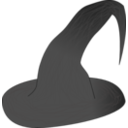
\includegraphics[scale=0.1]{bars4.png}}}


% custom dates
\usepackage{datetime2}


%\newlength{\outerbordwidth}
\raggedbottom
%\raggedright

\usepackage{framed}
\usepackage{tocloft}
\usepackage{multicol} % for the multiple column'd list


%Margin setup

\usepackage{geometry}

%\setlength{\evensidemargin}{-0.25in}
\setlength{\headheight}{0in}
\setlength{\headsep}{0in}
\setlength{\oddsidemargin}{-0.25in}
\setlength{\paperheight}{11in}
\setlength{\paperwidth}{8.5in}
\setlength{\tabcolsep}{0in}
\setlength{\textheight}{9.3in}
\setlength{\textwidth}{7in}
\setlength{\topmargin}{-0.3in}
\setlength{\topskip}{0in}
%\setlength{\voffset}{0.1in}
\setlength{\parindent}{0in}
\setlength{\itemsep}{0pt}

% unindented lists
\usepackage{enumitem}

% compress line spacing
\usepackage{setspace}
%\setstretch{0.9}
%\halfspacing

% fancy font for skills
\usepackage{fetamont}
\usepackage[T1]{fontenc}

% symols
\usepackage{fontawesome}

%% the footer
\usepackage{lastpage}
\usepackage{fancyhdr}
\pagestyle{fancy}
\renewcommand{\headrulewidth}{0pt}  % gets rid of horizontal rule in header
\rhead{\textit{updated \Today}}
\cfoot{\faGithubAlt~\href{https://github.com/crypdick}{crypdick}  $\cdot$ \faLinkedin~\href{https://www.linkedin.com/in/richarddecal/}{richarddecal} $\cdot$ \faStackOverflow~\href{https://stackoverflow.com/users/4212158/crypdick}{crypdick}  $\cdot$ \faHome~\href{http://www.richarddecal.com}{homepage}  \\ \faEnvelope ~\href{mailto:decal@uw.edu}{decal@uw.edu}  $\cdot$ \faPhone~ +1 48448-DECAL $\cdot$ \faMapMarker~St. Petersburg, FL, USA } % except the center \\
\rfoot{\thepage/\pageref{LastPage}}

%Grey heading bars
\usepackage[svgnames]{xcolor}
\definecolor{mygrey}{gray}{0.94}
\newcommand{\resheading}[1]{{\vspace*{.06in} \colorbox{mygrey}{\begin{minipage}{\textwidth}{\textmd{\large \textbf{#1} \vphantom{p\^{E}}}}\end{minipage}}} }

% job sections
\newcommand{\ressubheading}[4]{
        \textbf{#1} \hfill #2\\
        \textit{#3} \hfill #4 \\}

%\renewcommand*\descriptionlabel[1]{\hspace\labelsep\emph{#1 -}}

% colored hyperlinks
\usepackage{hyperref}
\hypersetup{
    colorlinks=true,
    linkcolor=black,    
    urlcolor=cyan,
    breaklinks=true
}
    \usepackage[hyphenbreaks]{breakurl}

\usepackage{ltablex}
%%%%%%%%%%%%%%%%%%%%%%%%%%%%%%%%%%%%%%%%%%%%%%%%%%%%%%%%%%%%%%%%%%%%%%%%%%%%%%%%%%
%%%%%%%%%%%%%%%%%%%%%%%%%%%%%%%%%%%%%%%%%%%%%%%%%%%%%%%%%%%%%%%%%%%%%%%%%%%%%%%%%%
%%%%%%%%%%%%%%%%%%%%%%%%%%%%%%%%%%%%%%%%%%%%%%%%%%%%%%%%%%%%%%%%%%%%%%%%%%%%%%%%%%
%%%%%%%%%%%%%%%%%%%%%%%%%%%%%%%%%%%%%%%%%%%%%%%%%%%%%%%%%%%%%%%%%%%%%%%%%%%%%%%%%%
\begin{document}

{\Huge Richard Boeri Decal} \\

%\begin{tabular*}{7in}{l@{\extracolsep{\fill}}r}
%\textbf{\Huge Richard Boeri Decal}%   \\

 
%\end{tabular*}
%\\
%\\


%%%%%%%%%%%%%%%%%%%%%%%%%%%%%%
\resheading{~\faGraduationCap~ Education}

    \ressubheading{Artificial Intelligence Engineer Nanodegree}{\href{https://www.udacity.com/nanodegree}{Udacity.com}}{Udacity \& Kaggle}{Jan. 2017 $\rightarrow$ Now}
 
    \ressubheading{B.A., Chemistry/Biology (Honors)}{Sarasota, FL}{New College of Florida}{Aug. 2007 $\rightarrow$ May 2011}
   % Thesis: ``Ebbs and Glows: Quantifying Small RNA Concentrations in \textit{C. elegans}''\\

  %  \ressubheading{Harriet L. Wilkes Honors College}{Jupiter, FL}{Early admission in lieu of a high school senior year}{Sep. 2006 $\rightarrow$ May 2007}

%%%%%%%%%%%%%%%%%%%%%%%%%%%%%%
\resheading{~\faTerminal~ Skills \hfill \small{Novice \OneBar $\cdot$ Intermediate \TwoBar $\cdot$ Proficient \ThreeBar $\cdot$ Master \FourBar }} 

\begin{tabularx}{\textwidth}{p{3.5cm}>{\arraybackslash}X}
  {\ffmfamily\bfseries{Algorithms}} & Regression \OneBar $\cdot$ gradient descent \ThreeBar $\cdot$ cross-validation \OneBar $\cdot$ \mbox{neural style transfer \ThreeBar} \\
  {\ffmfamily\bfseries{Languages}} & Python \ThreeBar $\cdot$ Bash  \OneBar $\cdot$ CSS \OneBar \\
  {\ffmfamily\bfseries{Programming}} & Pandas  \ThreeBar $\cdot$ Numpy  \ThreeBar $\cdot$ Scikit-learn  \OneBar $\cdot$ Matplotlib  \TwoBar $\cdot$ Git \TwoBar $\cdot$ \mbox{Unix CLI \TwoBar} $\cdot$  MySQL \OneBar \\
  {\ffmfamily\bfseries{OS}} & Linux \ThreeBar $\cdot$ MS Windows \ThreeBar $\cdot$  Mac OS X \ThreeBar $\cdot$ Android \FourBar $\cdot$ iOS \TwoBar \\
  {\ffmfamily\bfseries{Research }} &  Former research in the fields of computational neuroscience, biochemistry, genetics, and marine biology. I am co-author on several peer-reviewed scientific publications.\\
  {\ffmfamily\bfseries{Misc.}} & Espa\~nol \ThreeBar $\cdot$ English \FourBar $\cdot$ Italian \TwoBar  $\cdot$ Mandarin \OneBar  $\cdot$ \LaTeX \TwoBar  $\cdot$  Photoshop \& Lightroom \ThreeBar  $\cdot$ Algorithmic financial trading \OneBar  $\cdot$ ZFS \OneBar $\cdot$ PGP \& Tor \ThreeBar $\cdot$ \mbox{Building computers \TwoBar} 
\end{tabularx}


%%%%%%%%%%%%%%%%%%%%%%%%%%%%%%
\resheading{~\faCodeFork~ Projects}

\begin{tabularx}{\textwidth}{p{3.5cm}>{\arraybackslash}X}
{\ffmfamily\bfseries{\href{https://github.com/crypdick/RoboSkeeter}{Roboskeeter }}} & Dynamical agent models of mosquito decision-making. Implemented in Python using Numpy, Pandas, Matplotlib, and Scipy.\\
\end{tabularx}

%
%\ressubheading{\hypertarget{Mosquitogrant}Multisensory Integration in Mosquitos}{Seatle, WA}{Fairhall Lab, University of Washington}{Oct. 2014 $\rightarrow$ Now}
%I create agent-based dynamical models of mosquito flight behavior and benchmark the models against wind-tunnel behavioral data.\\ % These models will be further validated using electrophysiological \& tethered flight data to test theories about multi-modal decision making.\\
    
% \ressubheading{\hypertarget{whalevolunteering}Humpback Whale Census}{James Price Point, Australia}{Kimberley Community Whale Research Project}{Aug. 2012 $\rightarrow$ Oct. 2012}
%    A community-initiated peer-review at the proposed site of the world's second-largest liquefied gas processing port. This peer-review's estimates of humpback migration and breeding activity near James Price Point revealed gross discrepancies in the original oil conglomerate's survey.  \\ %old link\href{http://tinyurl.com/JPP-humpback-whale-survey-2013}{peer-review}'s

%    \ressubheading{Honors Baccalaureate Thesis}{Sarasota, FL}{Walstrom Lab, New College of Florida}{Aug. 2010 $\rightarrow$ May 2011}
%   My capstone \hyperlink{thesispub}{thesis project} proposes a model for RNA Helicase A function in endogenous \emph{C. elegans} RNAi pathways.\\ % My baccalaureate exam was administered by a committee of faculty and consisted of a thesis defense followed by a comprehensive oral exam covering all courses I took at New College.\\

%    \ressubheading{Tutorials}{Sarasota, FL}{New College of Florida}{Aug. 2007 $\rightarrow$ May 2011}
%    I created classes using New College's tutorial system, in which students are able to design courses in collaboration with faculty. Highlights: ``Wikipedia: Community, Technology, Society", ``Quantitative RT-PCR", ``Arduino Programming", ``Floridian Invasive Species", and ``Organic Lab Research".\\

%    \ressubheading{Genomics Outreach for Minorities Project (NSF-REU)}{Seattle, WA}{Pallanck Lab, University of Washington}{May 2010 $\rightarrow$ Aug. 2010}
%    I helped establish a method to grow, stain, and image primary dopaminergic neural culture from \textit{Drosophila} embryos in order to test whether Parkin and PINK1, proteins involved in Parkinson's disease, are recruited to depolarized mitochondria in dopaminergic neurons. This research was \hyperlink{neuronpub}{published} in \textit{PNAS}.\\

%    \ressubheading{Lab Technician}{Sarasota, FL}{New College of Florida Dept. of Natural Sciences}{Feb. 2010 $\rightarrow$ Sep. 2010}
%    Routine duties for the department, including autoclaving and disposing lab waste, preparing and sterilized solutions and agar plates, and preparing lab courses as needed. \\

%    \ressubheading{Organic Lab Research Tutorial}{Sarasota, FL}{Scudder Lab, New College of Florida}{Sep. 2008 $\rightarrow$ Nov. 2009}
%    I partially synthesized precursors to a novel high-valent iron-stabilizing macrocycle based on the active site of cytochrome P450.\\ % My work was summarized in a paper entitled, ``Towards Synthesis of a Cytochrome P450 Mimic".\\ % A continuation of New College graduate Dan Kaplan's thesis research.

%    \ressubheading{Summer Undergraduate Research Program (NSF-REU)}{Pittsburgh, PA}{McCartney Lab, Carnegie Mellon University}{May 2009 $\rightarrow$ Aug. 2009}
%    I determined that APC2, a protein with probable roles in colon cancer tumorogenesis, did not interact with $\beta$-catenin of the Wnt pathway's destruction complex. I determined that APC2's conserved N-terminal domain was not essential for its proper localization. This research was \hyperlink{carnegiepub}{published} in \textit{Genetics}.\\
%    
%    \ressubheading{Independent Study Project}{Sarasota, FL}{New College of Florida}{Jan. 2009}
%    A 4-week project conducted under the direction of Dr.\ Necmettin Yildirim. Using MATLAB, we modelled biological and chemical systems, particularly oscillating kinetic systems such as the Brusselator.\\ % I presented my work in a seminar entitled, ``Modelling the Dynamics of Life".\\
%
%    \ressubheading{Independent Study Project}{Sarasota, FL}{McCord Lab, New College of Florida}{Jan. 2008}
%    I studied chromatographic theory and operated gas and high-pressure liquid chromatographs.\\ % I researched and isolated triclosan, a ubiquitous bactericide and suspect carcinogen.\\

%%%%%%%%%%%%%%%%%%%%%%%%%%%%%%%
%\resheading{Publications}
%
%    %\textbf{Academic}
%    
%     \hypertarget{neuronpub} Burman JL, Yu S, Poole AC, \textbf{Decal RB} and Pallanck LJ. ``\href{http://www.pnas.org/content/early/2012/06/12/1120688109}{Analysis of neural subtypes reveals selective mitochondrial dysfunction in dopaminergic neurons from parkin mutants}". \textit{Proc Natl Acad Sci USA.} 2012 Jun 26;109(26):10438-43. \\            
%    
%      \hypertarget{carnegiepub} Kunttas-Tatli E, Zhou M, Zimmerman S, Molinar O, Zhouzheng F, Carter K, Kapur M, Cheatle A, \textbf{Decal R}, McCartney BM. ``\href{http://www.genetics.org/content/190/3/1059.full}{Destruction Complex Function in the Wnt Signaling Pathway of Drosophila Requires Multiple Interactions Between Adenomatous Polyposis Coli 2 and Armadillo}". \textit{Genetics}. 2012 Mar; 190(3):1059-75.\\    
%    
%%       \hypertarget{thesispub} \textbf{\textbf{Decal RB}}. ``\href{http://tinyurl.com/RichardDecal-NCF-Thesis}{Ebbs and Glows: Quantifying Small RNA Concentrations in \textit{C. elegans}}". Honors thesis, New College of Florida. May 2011. 108 pages.\\
\resheading{~\faBriefcase~ Experience}

%\ressubheading{Owner and Creator Assistant}{Seatle, WA}{Light Recycled}{Oct. 2014 $\rightarrow$ Jan. 2016}
%\begin{itemize}[noitemsep,topsep=0pt,parsep=0pt,partopsep=0pt, nolistsep]
%\item Created simulations of mosquito decision-making experiments using SciPy.
%\item Preparing manuscript for peer-review.
%\end{itemize}

\ressubheading{Research Assistant}{Seatle, WA}{Fairhall Lab, Dept. of Biophysics, Uni. of Washington}{Oct. 2014 $\rightarrow$ Jan. 2016}
\begin{itemize}[noitemsep,topsep=0pt,parsep=0pt,partopsep=0pt, nolistsep]
\item Created simulations of mosquito decision-making experiments using SciPy.
\item Preparing manuscript for peer-review.
\end{itemize}
 
\end{document}